\begin{frame}{Workflow: Stagin area and commit}
\footnotesize

\onslide<2->{
\begin{block}{Adding files to staging area}
\begin{semiverbatim}
\$ git add file.txt



%\only<3->{
%Noch keine Commits
%
%Unversionierte Dateien:
%  (benutzen Sie "git add <Datei>...", um die Änderungen zum Commit vorzumerken)
%	file.txt
%
%nichts zum Commit vorgemerkt, aber es gibt unversionierte Dateien
%(benutzen Sie git add zum Versionieren)
%}
\end{semiverbatim}
\end{block}
}

\onslide<3->{
\begin{block}{Commit}
\begin{semiverbatim}

\$ git commit



\end{semiverbatim}
\begin{center}
\only<4>{
 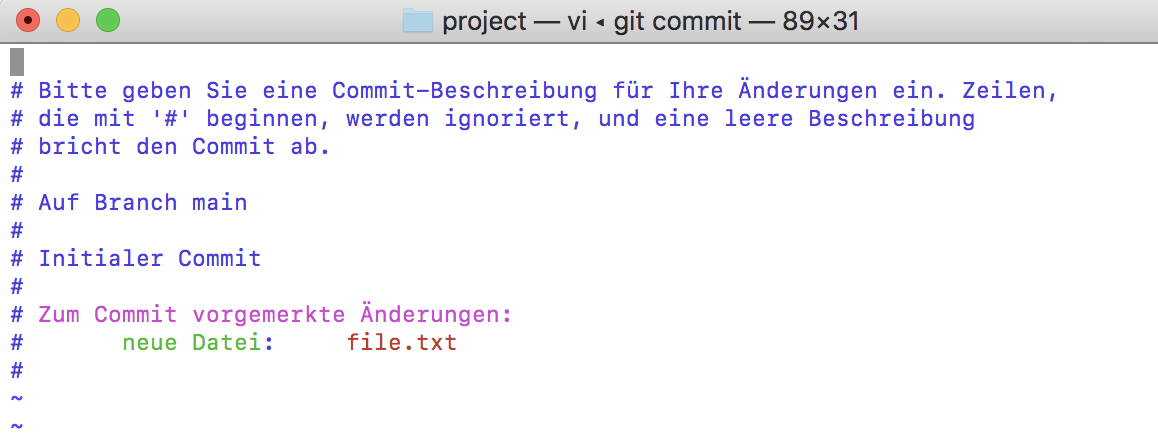
\includegraphics[width=0.8\textwidth]{pics/commit.png}
}
\end{center}
\end{block}
}

\end{frame}
